\chapter{Embedding Methods}
\label{chap:emb}
\section{Introduction}
The electronic structure methods outlined in the previous chapter all succeed in achieving increased accuracy with greater computational cost. In the case of chemical processes in condensed phases, the amount of electrons representing every actor in the process becomes unmanageably large.

Fortunately, oftentimes, the process of interest is confined to a local area within the material. We may therefore adopt the strategy of selecting a molecular sample from the system, and performing calculations on this subsystem. Of course, the interaction of the environment with the subsystem can be determining in the process under study, and therefore often needs to be reflected in the computational simulation.

\section{Polarisable Continuum Models}
The first approximation to the environmental interactions between a solvent or crystal and a local site, is that of directly applying a model potential to the Hamiltonian of the quantum description of that site. This is in contrast to later discussed methods which explicitly represent the environment of the area of interest. As such, in the current case, the molecules under scrutiny are said to be placed in a \textit{continuum}, and the large family of implicit solvation models are also called continuum models.\cite{Tomasi2005}

As a general rule, continuum models partition the simulation space between a cavity, which contains a large portion of the electron density of the simulated molecule, and an infinite environment, meant to represent the medium. An effective method to reflect the electrostatic potential of the medium, is to reduce it to a potential on the surface of the cavity. The potential within the cavity is related to the surface charge $\sigma(\bm{s})$ as follows:\cite{Mennucci2012}

\begin{equation}
    V_{\sigma}(\bm{r}) = \int_{\Gamma} \frac{\sigma(\bm{s})}{\abs{\bm{r}-\bm{s}}} d\bm{s}
\end{equation}
Where we are integrating over the surface of the cavity $\Gamma$. The correct form of $\sigma(\bm{s})$ determines the quality of this kind of continuum model. If we presume that the inner and outer regions of the cavity have different but isotropic dielectric permittivities, we can derive a surface charge:\cite{Miertus1981}

\begin{equation}
    \sigma (\bm{s}) = \frac{\epsilon - 1}{4\pi \epsilon} \frac{\partial}{\partial \bm{n}} (V_M(\bm{s}) + V_{\sigma}(\bm{s}))
    \label{eq:surface_charge}
\end{equation}

Where the $\epsilon$ is the medium's dielectric constant, $V_M(\bm{\sigma})$ and $V_{\sigma}(\bm{\sigma})$ are the electrostatic potentials emanating from the inner region charge density and the surface charge, and $\bm{n}$ is the unit vector normal to the surface at point $\bm{s}$. The surface charge is a function of its own potential, making Equation \ref{eq:surface_charge} require self-consistent calculations to solve.

This method is known as the Dielectric Polarisable Continuum Model (DPCM, sometimes PCM). It has the advantage that it does not require additional explicit molecular calculations to evaluate the solvation properties of the sample, and the solvent is defined by a tunable dielectric constant. However it ignores non-electrostatic interactions, which are key to the structure of dense condensed phases. Moreover, it presumes an isotropy which, loses the ordered property of the Coulomb environment in crystal materials.

\section{Point Charge Embedding}
\label{sec:pce}
\subsection{Non-isotropic Media}
The electrostatic interactions between a molecular system and its environment can indeed be highly directional. In molecules with an asymmetric polarity, the periodic stacking of their crystal form means that one side of the molecule will be in closer contact with electronegative atoms than the other. Thus, instead of using a continuum, it would be useful to locate the sources of electrostatic potential\textemdash{}the environment atoms\textemdash{}in space.

Given a certain partial charge $q_i$ on an environment atom at position $\bm{R_i}$, one can use atom centred point charges to represent the total electrostatic potential of the medium as such:
\begin{equation}
    V^{\text{ES}}(\bm{r})=\sum_i \frac{q_i}{\abs{\bm{r}-\bm{R_i}}}
    \label{eq:point_char}
\end{equation}
If we embed the system's Hamiltonian in the above potential, we can make its electron density respond to the environmental Coulomb potential.

Note that this scheme does not include any non-Coulombic forces, giving it a very poor description of short range interatomic interactions. Furthermore, while in the long range limit, the electrostatic potential from an atom does tend towards an inverse law, it does not have the infinite growth at $\bm{r} = \bm{R_i}$ which exists in Equation \ref{eq:point_char}. It, instead, shows a finite cusp centred about the nucleus, called Kato's cusp, whose value depends on the charge of the nucleus.\cite{Kato1957,March1986}

Thus, we must be aware that the accuracy of the electrostatic potential emanating from point charges deteriorates as the distance from the nucleus becomes small. We call the error in electronic calculations caused by this discrepancy \textit{overpolarisation}.\cite{Biancardi2016} In such cases, with the point charge potential being infinitely attractive, the simulated charge density can be funnelled to the nuclear position. It is therefore important to choose a basis set which does not allow the wavefunction of the molecular system to extend onto nuclear positions in the environment.

\section{General QM:MM}
\subsection{Cluster Models}

An alternate method for modelling a multiscale system is by explicitly modelling the environment at a lower level of theory than the site of interest. This defines the family of \textit{hybrid} methods, which combine different quantum or classical methods into one.
At this point, it becomes important to concretise what would take the role of the central region and environment in the case of molecular crystals. Thankfully, the non-covalent nature of these materials offers us an inherent partition.

If we care about a process localised on a few neighbouring molecules, then they become the high level of theory region (region $\bm{1}$), and a surrounding cluster of molecules taken from their crystal position becomes the low level of theory region (region $\bm{2}$). This partition is represented on Figure \ref{fig:benz_clu} for the case of a cluster of benzene molecules where the active site is one unit. The size and shape of this cluster is a topic of discussion, but the smallest useful one would include all of the nearest neighbours to the region $\bm{1}$ molecules, ensuring an isotropic coverage of the short range interactions.

\begin{figure}
\centering
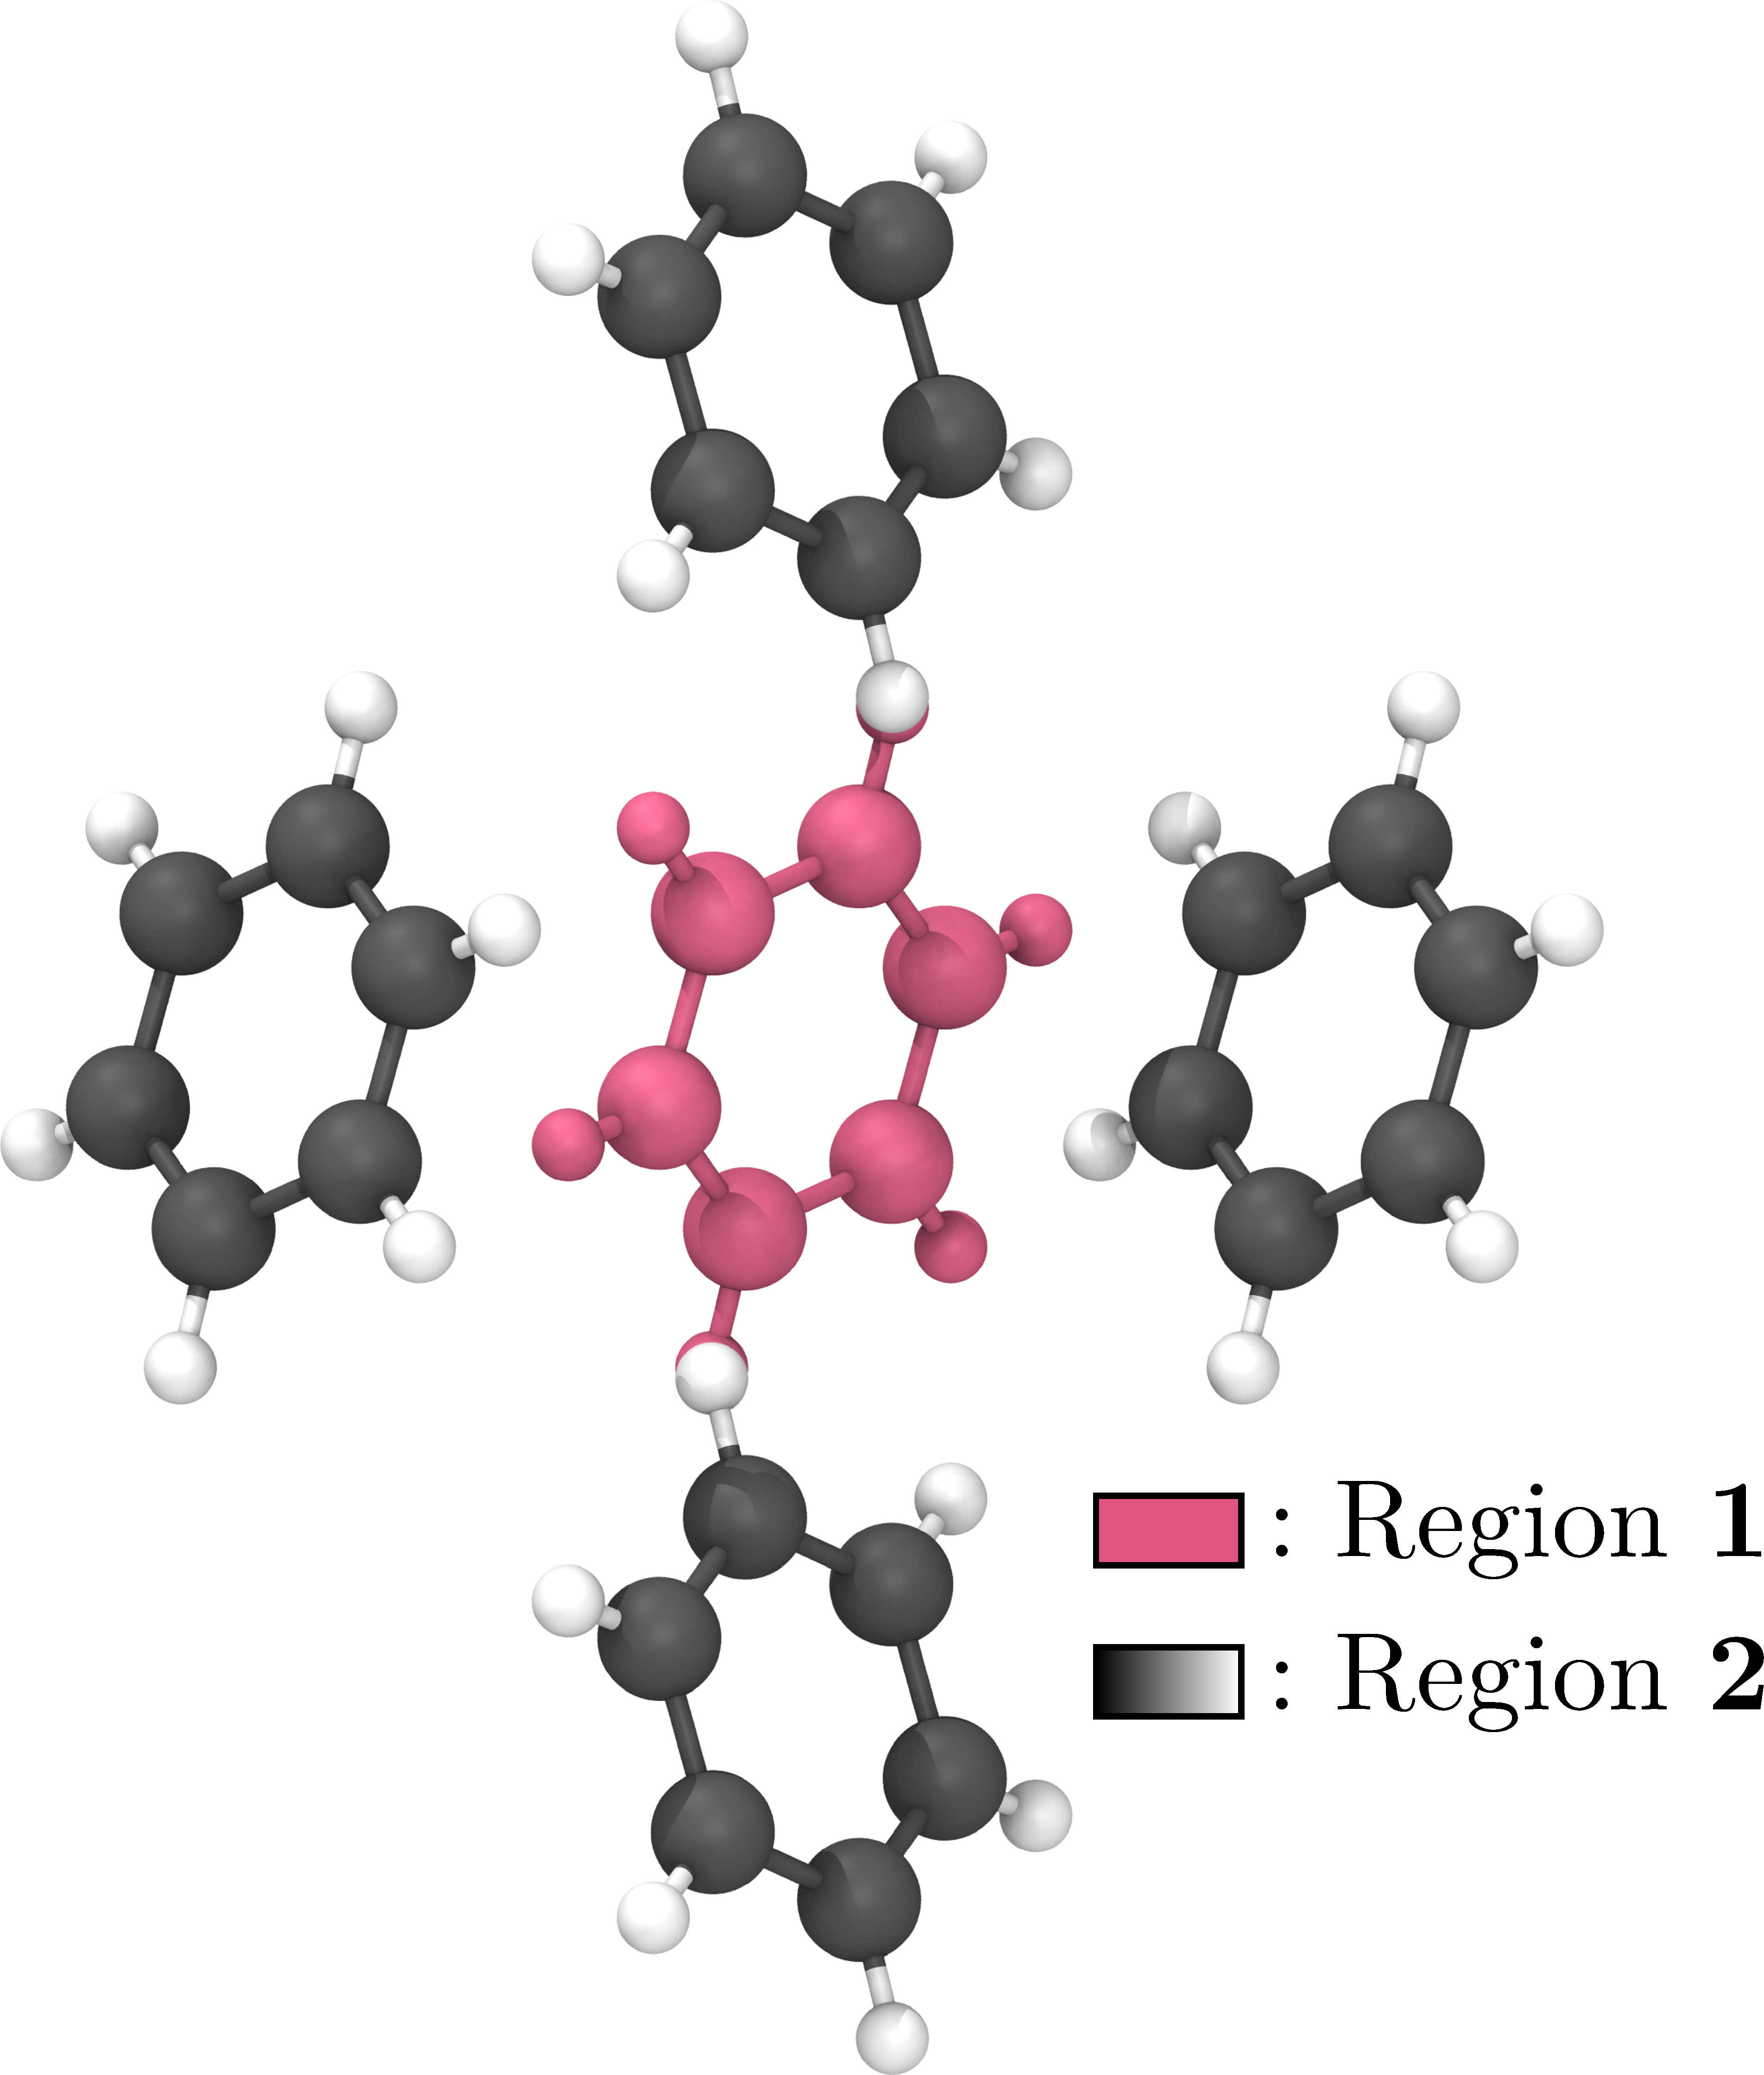
\includegraphics[width=7cm]{Chapters/3Embedding/benz_example_cluster.pdf}
\caption{Example of a cluster of benzene atoms taken from their lattice positions. The pink molecule denotes the central region.}
\label{fig:benz_clu}
\end{figure}

As a side note, if we wanted to partition the cluster through a covalent bond, we would terminate the dangling bonds of region $\bm{1}$ and potentially $\bm{2}$ with appropriate fictitious monovalent atoms. This explains why in certain scenarios, region $\bm{1}$ is referred to as \textit{model} system, in the literature. We forego this convention, since this discussion is centred around system-environment boundaries which do not cleave bonds.

\subsection{Intermolecular Interactions}
Our main goal now consists in modelling the energy of region $\bm{1} \cup \bm{2}$. We can write:
\begin{equation}
    E_{\text{high}:\text{low}}(\bm{1} \cup \bm{2}) = E_{\text{high}}(\bm{1}) + E_{\text{low}}(\bm{2}) + E^{\text{int}}_{\text{high}:\text{low}}(\bm{1},\bm{2})
    \label{eq:generic_hybrid}
\end{equation}
Where $E_{l}(\bm{n})$ is the energy of the isolated region $\bm{n}$, at the level of theory $l$, and $E^{\text{int}}_{\text{high}:\text{low}}(\bm{1},\bm{2})$ is the interaction energy between the two regions. The first developed hybrid methods, and still the most popular today, were those combining quantum mechanics methods with molecular mechanics methods (QM:MM). We can rewrite Equation \ref{eq:generic_hybrid} with QM:MM indices:\cite{Warshel1976}

\begin{equation}
    E_{\text{QM}:\text{MM}}(\bm{1} \cup \bm{2}) = E_{\text{QM}}(\bm{1}) + E_{\text{MM}}(\bm{2}) + E^{\text{int}}_{\text{QM}:\text{MM}}(\bm{1},\bm{2})
    \label{eq:generic_qmmm}
\end{equation}
 The crux of QM:MM techniques relies in finding an appropriate expression for $E^{\text{int}}_{\text{QM}:\text{MM}}(\bm{1},\bm{2})$. The family of methods which focus on calculating the first two terms of Equation \ref{eq:generic_qmmm} with electronic structure and molecular mechanics packages, and then computing the interaction term explicitly are called \textit{additive} QM:MM.

\section{IMOMM}
A parallel family of methods uses a different formulation, instead choosing to implicitly consider the interaction term \textit{via} a subtraction. First, we consider the components of the energy of the whole system in at the MM level of theory:
\begin{equation}
    E_{\text{MM}}(\bm{1} \cup \bm{2}) = E_{\text{MM}}(\bm{1}) +  E_{\text{MM}}(\bm{2}) + E^{\text{int}}_{\text{MM}}(\bm{1},\bm{2})
\end{equation}{}

We can reorder this as $E_{\text{MM}}(\bm{2}) + E^{\text{int}}_{\text{MM}}(\bm{1},\bm{2}) = E_{\text{MM}}(\bm{1} \cup \bm{2}) - E_{\text{MM}}(\bm{1})$, and insert it in Equation \ref{eq:generic_qmmm}, provided that we only require an MM level description of the interaction energy. The full Integrated Molecular Orbital Molecular Mechanics (IMOMM), energy is finally written:\cite{Maseras1995}

\begin{equation}
    E^{\text{ONIOM}}_{\text{QM}:\text{MM}}(\bm{1} \cup \bm{2}) = E_{\text{QM}}(\bm{1}) + E_{\text{MM}}(\bm{1} \cup \bm{2}) - E_{\text{MM}}(\bm{1})
    \label{eq:imomm}
\end{equation}
The meaning of the term ``ONIOM'', is explained later. The energy gradients can naturally be calculated in the same way. For instance the force on region 1 atoms is the negative of the following:

\begin{equation}
    \frac{dE^{\text{ONIOM}}_{\text{QM}:\text{MM}}(\bm{1} \cup \bm{2})}{d\bm{1}} = \frac{dE_{\text{QM}}(\bm{1})}{{d\bm{1}}} + \frac{dE_{\text{MM}}(\bm{1} \cup \bm{2})}{d\bm{1}} - \frac{dE_{\text{MM}}(\bm{1})}{d\bm{1}}
    \label{eq:imomm_grad}
\end{equation}

Let us carefully compare Equations \ref{eq:generic_qmmm} and \ref{eq:imomm}. In the former, only one MM calculation is carried out, as opposed to two in the latter, including one necessarily larger one ($\bm{1}\cup\bm{2}$). In our case, this is not a significant issue, since we will wish to push the accuracy of the QM level of theory, making it, and not any MM calculations, the computational bottleneck of the method.

We have also gotten rid of any explicit calculation of the interaction term. This is a promising feature, since the components of the intermolecular interaction are difficult to express and disentangle, however we are now left with the inter-region interactions reflected only by their MM description.

\section{QM:MM Electrostatic Embedding}
One significant issue of the MM description of inter-region interactions is that they do not capture any electronic response from the region $\bm{1}$ atoms to the environment at a quantum level of theory. This is a particularly severe shortcoming for electrostatic interactions, which are far-reaching by nature, and can determine the electronic structure of the investigated ground or excited states.

To overcome this difficulty, the inter-region electrostatic energy in the second term of Equation \ref{eq:imomm} must be removed\textemdash{}this is a known quantity in MM calculations\textemdash{}and injected in the first term. This method is called \textit{electrostatic embedding}, and hybrid methods without it are said to use \textit{mechanical embedding}. The most common electrostatic embedding method complements the QM Hamiltonian of region $\bm{1}$ with point charges at the location of region $\bm{2}$ atoms, with charge values determined by the forcefield. This allows the electron density of region $\bm{1}$ to respond to the electrostatic potential of the environment, as is discussed in Section \ref{sec:pce}.

\section{ONIOM QM:QM'}

If we want to increase the level of accuracy of the inter-region interactions, while still using a subtractive scheme, we must use a better low level of theory than MM. The Integrated Molecular Orbital Molecular Orbital (IMOMO) method, does just this, yielding an energy equation of the form:\cite{Humbel1996}
\begin{equation}
    E^{\text{ONIOM}}_{\text{QM}:\text{QM}'}(\bm{1} \cup \bm{2}) = E_{\text{QM}}(\bm{1}) + E_{\text{QM}'}(\bm{1} \cup \bm{2}) - E_{\text{QM}'}(\bm{1})
    \label{eq:imomo}
\end{equation}
Where QM' is a quantum level of theory lower in accuracy than QM. At this point, it is worth mentioning that these hybrid method schemes can be extended to include as many regions and methods as necessary. The general term for subtractive schemes, regardless of number of layers and type of modelling method, is \textit{our own n-layered integrated molecular orbital and molecular mechanics} (ONIOM).\cite{Svensson1996} ONIOM is a superset of IMOMM and IMOMO, and we therefore employ it in our energy expressions since specifying the levels of theory involved renders the distinction between IMOMM or IMOMO superfluous.

If we want to keep using electrostatic embedding for IMOMO, the implementation is more delicate than for IMOMM. Here, the inter-region Coulomb interaction is not a known quantity which could be removed from the second term of Equation \ref{eq:imomo}. Instead, we must embed the third term in point charges, thus cancelling out the electrostatic interaction present in the second. A discussion of the choice of point charge can be found in Chapter \ref{chap:jctc}.

\section{Shortcomings of ONIOM Embedding Methods}
\label{sec:problems}
This section serves as a motivation for the rest of the work presented in this thesis. As such, some of the problems of ONIOM methods are briefly discussed now, and are addressed in Chapter \ref{chap:jctc}.

\subsection{Inclusion of Long-Range Effects}
\label{sec:prob_lr}
In ONIOM schemes, region $\bm{1}$ is subject to the environmental interaction of region $\bm{2}$. A region $\bm{2}$ containing only the nearest neighbour molecules should suffice to cover the non-electrostatic effect, owing to their short-range nature.\cite{Fornari2017} However electrostatic effects decay as an inverse law, and therefore can have a significant impact on the electronic state of region $\bm{1}$.

It is unclear how many layers of molecules in region $\bm{2}$ would suffice to represent the screened electrostatic potential in an amorphous material, but the larger the region, the higher the cost to model computationally. Moreover, as discussed in Section \ref{sec:ewald}, in a crystal, the accuracy of the potential does not systematically improve with a larger region, making traditional ONIOM a poor choice if long-range effects have a role in the system under study.

\subsection{Point Charge Representation}
\label{sec:prob_char}
The use of point charge embedding to represent electrostatic effects presumes a similarity between the Coulomb potential of a point charge and that of an atomic charge density. We have already discussed a discrepancy in the short-range in Section \ref{sec:pce}, but how can we ensure that the point charge values which we employ for each atom will have the correct behaviour in the mid-to-long-range?

Indeed, there is no absolute definition of an atom's partial charge, and the variety of population analysis schemes available to use suggests that some will be more appropriate than others in representing the electrostatic potential of the atom for the embedding of region \textbf{1} at high and low levels of theory. A successful scheme, combined with valid electronic structure methods, would reproduce accurate absorption and emission energies of molecules in their crystal environment, whilst fulfilling an appropriate cancellation of errors in the ONIOM equation.

A commonly used method for both is that of the Mulliken analysis,\cite{Hratchian2008} which essentially accounts for the contribution of individual atomic orbitals to the overall electron density, and then sums up this contribution between all the orbitals belonging to one atom.\cite{Mulliken1955}

Some known problems are the fact that the electron population being shared between two orbitals of different atoms will necessarily be split in half, not accounting for the potential discrepancy between the electron affinity of the nuclei. Furthermore, due to being directly defined by the basis set of the calculation, Mulliken charges are highly basis set dependent. For instance the charge values on a water molecule can vary up to 0.7 $\mathrm{e^-}$ depending on the basis set.\cite{Martin2005}

It is therefore unclear whether the most commonly used partial charge scheme is appropriate for electrostatic embedding. We ought to seek out alternatives, and compare the effect of their embedding on the electronic structure of region \textbf{1} molecules.

\subsection{Mutual Polarisation}
\label{sec:prob_sc}
The electrostatic embedding methods described above allow for the representation of the static Coulomb interaction of the crystal on the active site. This one-way relation is not an accurate representation of the real scenario where the regions \textbf{1} and \textbf{2} mutually polarise each other until they find an equilibrium at fixed nuclear coordinates, following the BO approximation.

Mutual polarisation plays an important role in certain excited state processes. For instance, the charge transfer states in LiF interacting with a Be atom were probed with different kinds of QM:MM implementations; and the non-polarisable one overestimated excited state energies by over 0.1 eV.\cite{hagras_polarizable_2018}. It is as of yet unclear how important these errors become in molecular crystals, and which methods should be employed to mitigate them. 

\subsection{Implementation}
\label{sec:prob_imp}
Finally, QM:QM' techniques face many issues in terms of their software implementation. On a technical level, the electronic structure programs which offer this feature are few and far between. Furthermore, each of those programs only implements a limited set of electronic structure methods, thus limiting the amount of QM and QM' method combinations available to the user. When modelling excited states, having as much flexibility as possible in the choice of method is crucial, due to the variety in character of many body excited state wavefunctions.

On a practical level, the task of selecting a region \textbf{1} and \textbf{2} combination, and assigning point charges to pertinent lattice positions is laborious, and difficult to incorporate in a reproducible workflow. For instance, \textit{nearest neighbour molecules} is a term with no formal definition, and while they can often be recognised at a glance, edge cases are certainly subjective to the researcher. An algorithmic method for the practical steps of setting up these calculations is therefore desirable.
